\documentclass[12pt,titlepage,figuresatend]{article}
%\usepackage[final]{JMR}
\usepackage{JMR}

\usepackage{authblk}
\renewcommand\Affilfont{\small}
%\renewcommand\Authands{, and }

\usepackage{lineno}
\linenumbers

\title{High-frequency variability in the\authorcr North Icelandic Jet}
%\author{First author\footnote{Address and email of first author} and Second Author\footnote{Address and email of second author}}
%\author[1]{First Author}
%\author[1]{Second Author}
%\author[1]{Third Author}
%\author[2]{Fourth Author}
%\affil[1]{Address of first author,\authorcr in two lines}
%\affil[2]{Address of second author in one lines}


\author{B. E. Harden\footnote{Woods Hole Oceanographic Institution, 266 Woods Hole Road, Woods Hole, MA 02543. bharden@whoi.edu}}
\author{R. S. Pickart}
%\author[2]{H\'{e}{\dh}inn Valdimarsson}
%\author[3]{Kjetil V{\aa}ge}
%\author[4,5]{Laura de Steur}
%\author[2,6]{Steingr\'{i}mur J\'{o}nsson}

\affil{Woods Hole Oceanographic Institution, Woods Hole, USA}
%\affil[2]{Marine Research Institute, Reykjavik, Iceland}
%\affil[3]{Geophysical Institute and Bjerknes Centre for Climate Research, \authorcr University of Bergen, Norway} 
%\affil[4]{Royal Netherlands Institute for Sea Research NIOZ, Texel, The Netherlands}
%\affil[5]{Norwegian Polar Institute, Troms{\o}, Norway}
%\affil[6]{University of Akureyri, Iceland}

\date{August 2017}

\begin{document}
\maketitle

\begin{abstract}
We describe the high-frequency variability in the North Icelandic Jet on the Iceland Slope using data from the densely instrumented K\"{o}gur array deployed upstream of the Denmark Strait sill from September 2011 to July 2012. Significant sub-8-day variability is ubiquitous in all moorings from the Iceland slope with a dominant period of 3.6 days. We attribute this variability to Topographic Rossby Waves on the Iceland slope with a wavelength of 62 $\pm$ 3 km and a phase velocity of 17.3 $\pm$ 0.8 km$\,$day$^{-1}$ directed downslope (-9$^{\circ}$T). We test the theoretic dispersion relation for these waves against our observations and find good agreement between the direction of phase propagation. We additionally calculate a theoretical group velocity of 36 km$\,$day$^{-1}$ directed almost directly up-slope (138$\,^{\circ}$T) which agrees well with the propagation speed of observed energy pulses headed upslope. We use a wave tracing model to show that this wave energy is generated locally, offshore of the array, and not in the upstream or downstream directions. We hypothesize that either the meandering Separated East Greenland Current at the foot of the Iceland slope or intermittent aspiration into the Denmark Striat Overflow are the drivers of the Topographic Rossby Waves. Regardless of the formation mechanism, the waves appear to be a local phenomena, not found in an instrumented record upstream.

\end{abstract}

\section{Introduction}

The Denmark Strait Overflow is the major pathway of dense water out of the Nordic Seas. It transports 3.2 Sv (or approximately 50\%) of the total outflow, which in turns allows for replenishment by poleward flowing warm surface waters \cite[]{Dickson1994,Jochumsen2017}. As such, the overflow plays a crucial role in the meridional overturning circulation, which moderates the climate of the North Atlantic. This has been known for many decades, but our understanding of the underlying dynamics requires much refinement.  Specifically, we need to know more about where the overflow water comes from and how it makes it’s way to the sill if we are to understand how shifting wind, sea ice and freshwater patterns will impact the efficiency of the Atlantic Meridional Overturning Circulation.

Most of the Denmark Strait Overflow water (approximately 70\%) comes from the East Greenland Current by ways of the Nordic Seas’ boundary current \cite[]{Vage2013,Harden2016} (see Figure \ref{mainmap}). Warm Atlantic inflow is progressively cooled as it circumnavigates this basin (and, to some degree, the Arctic Ocean) before sinking to mid-depth along the east coast of Greenland and flowing into the northern side of the Denmark Strait \cite[]{Mauritzen1996}. 

\begin{figure}[p!]
  \centering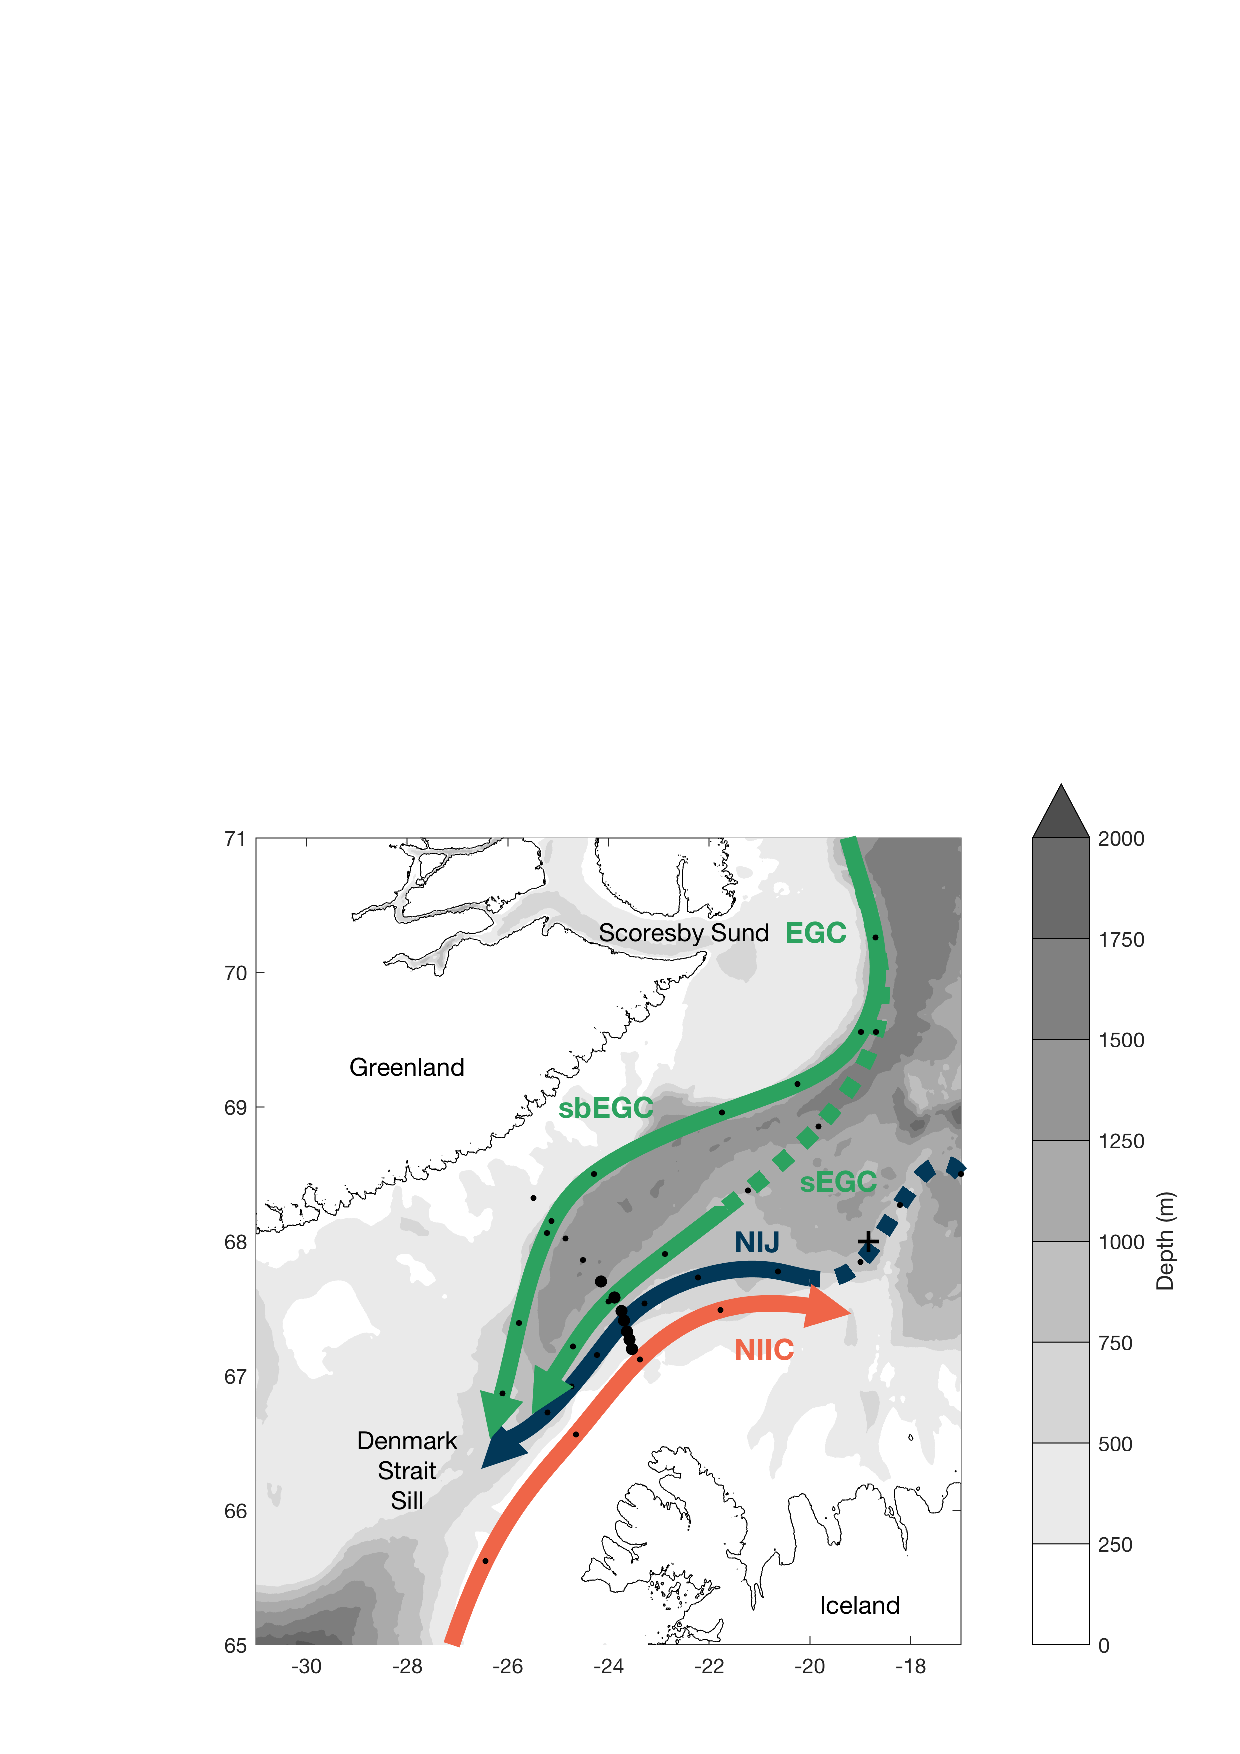
\includegraphics[width=.9\hsize]{./figures/mainmap.pdf}
  \caption{Map of study region showing the overflow pathways approaching the Denmark Strait Sill: the North Icelandic Jet (NIJ) and the two East Greenland Current (EGC) pathways, one along the shelfbreak (sbEGC) and the other in a separated branch on the Iceland Slope (sEGC). Dashed sections show parts of pathways that still in need of further clarification. Also shown is the northward flowing surface current, the North Icelandic Irminger Current (NIIC). Block dots show the locations of the moorings in the K\"{o}gur array with larger dots indicating the subset of seven moorings used in this study. The upstream cross is the mooring to the west of the Kolbensey ridge referred to in the text. The bathymetry is from IBCAO.}{\label{mainmap}}
\end{figure}

As the East Greenland Current rounds Scorsbysund, it splits into two branches (Figure \ref{mainmap}). One continues towards the sill as a shelf-break jet (HavikXXX). The other bring approximately 60\% of the overflow water out into the central strait through eddies and/or a gyre-like deflections of the shelf-break jet \cite[]{Vage2013,Harden2016}. This separated pathway brings overflow water from the East Greenland Current across the Strait and onto the Iceland Slope.

The remaining 30\% of Denmark Strait Overflow water comes by ways of the North Icelandic Jet, a relatively recently discovered branch of the upstream circulation \cite[]{Steingrimur2004,Vage2011}. The mid-depth intensified jet brings waters distinct from those found in the East Greenland Current (colder and fresher) suggestive of a unique source in the central Iceland or Greenland seas \cite[]{Vage2011,Vage2015,Harden2016}. It also contains the densest water that feeds the overflow; its waters are those found in the deepest part of the sill \cite[]{Mastropole2017} and therefore will sink to the deepest depths in the core of the overflow.

A leading hypothesis for the formation of the North Icelandic Jet, which has been supported by both models and observations, is via a local overturning cell in the Iceland sea; Atlantic inflow in the North Icelandic Irminger Current sheds warm water into the Iceland Sea, which undergoes deep convection, before returning towards the sill in the North Icelandic Jet \cite[]{Vage2011,Behrens2017}. However, many questions remain unanswered about this proposed system, not least of which is the general shallow nature of the winter mixed-layer throughout much of the Iceland Sea \cite[]{Vage2015} and the known formation of overflow water further north in the Greenland Sea \cite[]{Strass1993,Rudels2002}.

Regardless of the source of the North Icelandic Jet, it clearly constitutes a vital component of the circulation upstream of the sill. However, we know little about the dynamics which govern its flow towards the sill in the observational record. \cite{Harden2016} discuss the Jet's mean and seasonal contribution to the overflow and report that it exhibits much high-frequency variability without going into any great detail. The North Icelandic Jet was initially described by \cite{Steingrimur2004} as a mid-depth intensified flow which sits on the 650 m isobath, but more recently, Pickart XXX described multiple instances of the Jet bifurcating, moving to different isobaths, and coupling to the poleward flowing North Icelandic Irminger Current.

Observational studies of the North Icelandic Jet dynamics to date have necessarily relied upon synoptic surveys \cite[]{Steingrimur2004,Vage2011} + Pickart2017. In this study, we aim to describe the dynamics of the North Icelandic Jet through an instrumented array in place across the combined upstream circulation over the course of 11 months (Figure \ref{mainmap}).  Our goals are to describe the short-period variability and its underlying mechanics.


\section{Methods}

Data for this study come from the densely instrumented K\"{o}gur mooring array spanning the Denmark Strait approximately 200 km upstream of the sill. The array was deployed for 11 months from September 2011 to July 2012 and comprised 12 moorings (called KGA 1-12) equipped with instrumentation to measure both the hydrography and velocity of the water column from 50 m to the bottom. \cite{Harden2016} present a complete description of the moored data. The array captured the majority of overflow water (denser than 27.8 kg$\,$m$^{-3}$) passing through the Strait towards the sill.

For this study we are primarily using the gridded product described in \cite{Harden2016} at a resolution of 8km and 50 m. Due to our focus on the Iceland slope, we are using a subset of these data up to and including the location of mooring KGA 7, approximately 70 km from the Iceland shelf break. Mean velocity sections demonstrate that this portion of the array captures both the North Icelandic Jet and the majority of the Separated East Greenland Current (Figure \ref{fig_section}). For some analysis we also use the data on a mooring-by-mooring basis. All data has been de-tided with a 36-hour low-pass filter.

Additional data comes from a mooring located approximately 200 km upstream of the K\"{o}gur Array on the west side of the Kolbesney Ridge (68$^{\circ}$00'N, 18$^{\circ}$50'W, see Figure \ref{mainmap}) This mooring was deployed on the 1000 m isobath from September 2007 to mid-October 2008. A Moored Marine Profiler equipped with an Acoustic Current Meter recorder produced current profiles between the bottom and 100 m at 8 hour intervals. As with the K\"{o}gur data, we low-pass at 36-hours to remove the tidal components of the flow. This data is described in greater detail by \cite{Jonsson2012}.

Our wavelet analysis uses the jLab toolbox \cite[]{Lilly2017} with standard Morlet wavelets with $\gamma$=3 and $\beta$ = 2.

When implementing inverse wave tracing, we use the inverse model described by \cite{Meinen1993} and implemented by \cite{Pickart1995} for tracing of Topographic Rossby Waves in the Deep Western Boundary Current off Cape Hatterus. The method uses the topographic wave dispersion relation to calculate an initial group velocity and backtrack the wave one timestep. The wave parameters are then recalculated for the new bottom depth, slope and stratification and a new group velocity calculated which is used to further trace the wave.

Many of the required input parameters come directly from the moored data and are the same as those we use for the theoretical Topographic Rossby Wave dispersion relation calculations (see Section \ref{results}.\ref{TRWsec}.). In addition, we chose a characteristic water depth of 1000 m, a timestep of 30 mins and a total integration period of 48 hours.

For the bathymetry, we used the International Bathymetric Chart of the Arctic Ocean 30-arcsec gridded product \cite[]{Jakobsson2012}. To remove seamounts and other sharp topographic features we smoothed the bathymetry at 60 km (comparable to our measured Topographic Rossby Wave wavelength). In contrast to \cite{Pickart1995} who then fit splines to the data to be able to find the bottom depth and gradients at any location, we deemed out resolution to be high enough (and our smoothing window great enough) for us to simply linearly-interpolate for any location.

\section{Results}
\label{results}

As discussed in \cite{Harden2016}, the average velocity and hydrography in the region show the signatures of both the North Icelandic Jet and the Separated East Greenland Current although the features are merged in the mean (Figure \ref{fig_section}). The North Icelandic Jet is on the upper Iceland Slope and is characterized by a mid-depth intensified flow carrying the coldest, densest overflow water banked up on the slope. The Separated East Greenland Current is further offshore; its key features are a surface intensification and the transport of warmer, saltier overflow water at approximately 300 m. Onshore of both these currents, on the Iceland shelf, is the poleward flowing North Icelandic Irminger Current (see also Figure \ref{mainmap}).

\begin{figure}[p!]
  \centering\includegraphics[width=.9\hsize]{./figures/plot_section.pdf}
  \caption{Mean section of the through-array velocity (top), and median sections of temperature (middle) and salinity (bottom) for the duration of the 11 months of the array deployment. Overlaid in black contours for each plot is the mean density section with the 27.8 kg$\,$m$^{-3}$ isopycnal (the transition to Denmark Strait Overflow Water) highlighted. The view is looking upstream through the array with Iceland on the right. Positive velocities indicate equatorward flow. Horizontal black dashed line indicates the depth of the Denmark Strait sill downstream. Moorings are labeled with black triangles and average instrument location are shown by grey points. Bathymetry is from an underway echosounder.}{\label{fig_section}}
\end{figure}

That the two overflow currents are merged in the mean is largely due to the high degree of variability on weekly time-scales. The depth-integrated, through-array velocity shows purvasive pulsing through this portion of the Strait (Figure \ref{fig_hoff}a). The period of this pulsing in the North Icelandic Jet portion of the array is concentrated at sub-8-day periods with a maximum average energy at 3.6 days (Figure \ref{fig_waveSpec}). Variability at periods greater than 8 days are also apparent, but confined to specific times in January, March and May.

\begin{figure}[p!]
  \centering\includegraphics[width=\hsize]{./figures/hoff_vars.pdf}
  \caption{Hoffmuller plots from the gridded data of a) the depth-mean velocity (below 100 m, same for all plots), b) the 8-day high-passed, depth-mean velocity field resolved to the direction major axis of the local variance ellipse, and c) the wavelet amplitude at a 4 day period for the depth-mean velocity field. Black sloped guidelines are angled at the theoretical group velocity for our measured Topographic Rossby Waves (see text for details). NB: The data is saturated at $\pm$20 cm$\,$s$^{-1}$  due to the large event in November.}{\label{fig_hoff}}
\end{figure}

Offshore, in the East Greenland Current, we also see these short-period pulses in addition to more consistent longer-period variability (not shown) that was described by \cite{Harden2016} as being in part due to the variable upstream bifurcation of the East Greenland Current.

In this study we focus on describing the higher-frequency, sub-8-day variability. To achieve this, we used an 8-day butterworth filter to isolate the high-frequency variability. We tried other period filters from 4 days to 30 days, but 8 days drew out the peak high-frequency variability most effectively.

The variance ellipses of this high-frequency variability for each mooring are useful in characterizing different regimes across the array (Figure \ref{fig_ellipse}). At KGA1, in the North Icelandic Irminger Current, the variance ellipses are elongated along the mean flow indicative a current pulsing along its axis. At KGA 6 and 7, within the Separated East Greenland Current, the elongation of the variance ellipses are perpendicular to the mean flow demonstrating that this current undergoes meanders. However, In the North Icelandic Jet (KGA 2-4), the major axes of the variance ellipses are aligned at an oblique angle to both the mean flow and the underlying bathymetry. KGA 5 appears to be a transition region between conditions in the North Icelandic Jet and those in the East Greenland Current.

\begin{figure}[ht!]
  \centering\includegraphics[width=\hsize]{./figures/TRWwavelet.pdf}
  \caption{Top: Depth-averaged U (black) and V (gray) components of velocity for the nearest gridded location to mooring KGA 3. Bottom left: Wavelet spectrum of time series in top panel using Morlet wavelets. The color scale for this plot is at the top right. Bottom right: Mean wavelet amplitude over length of deployment. Dashed line in bottom panels shows the cut-off period for the high-pass filter used in this study.}{\label{fig_waveSpec}}
\end{figure}


\subsection{Topographic Rossby Waves}
\label{TRWsec}

We resolved the sub-8-day depth-averaged flow in the gridded product along the major axis of the variance ellipses at each offshore location. Particularly in the North Icelandic Jet, the variability along these axes have a sinusoidal form and are lagged between moorings such that the pulses of current move offshore in time (Figure \ref{fig_hoff}b). This implies a downslope phase propagation of this variability.

We argue that this comes from the existence of Topographic Rossby Waves (TRWs). TRWs are planetary waves that are supported by a topographic gradient and produce transverse wave variability that is often at an oblique angle to the mean flow. They are produced in many slope regions of the world’s oceans \cite[]{Garrett1979,Louis1982,Pickart1990}. Key features of TRWs include wave-vectors (and hence phase velocities) that are perpendicular to velocity variability, a group velocity which is at an oblique angle to the phase velocity, and a propensity to be bottom-trapped by stratification.

\begin{figure}[ht!]
  \centering\includegraphics[width=\hsize]{./figures/map_ellipse.pdf}
  \caption{Map of the mooring locations (black dots) with the mean velocity (thin black arrows) averaged from 100 m to the depth of the ADCP record at each mooring (see gray lines in Figure \ref{fig_section}). Ovals are the 8-day high-passed variance ellipses for the same depth range. Thick black arrow shows the Topographic Rossby Wave (TRW) phase velocity averaged over KGA 2-4 (plotted at KGA 3). The dashed black arrow is the calculated TRW group velocity. The long black line is the mean downslop direction averaged between KGA 2-4. Bathymetry is from IBCAO.}{\label{fig_ellipse}}
\end{figure}

Given that the phase propagation is perpendicular to the velocity variability, we can calculate that the wave phase is progressing downslope at -9$^{\circ}$T (average from moorings KGA 2--4, see Figure \ref{fig_ellipse}). Following \cite{Pickart1990}, we further calculated the phase speed over the range of moorings KGA 2--4 (where we clearly see the wave signal) using,

\begin{eqnarray*}
  c_p = \frac{1}{T}\, \frac{360}{\overline{\phi}}\, \frac{\overline{\Delta S}}{cos(\Delta)}
\end{eqnarray*}

where $T$ is the wave period (= 3.6 days), $\overline{\phi}$ is the average phase offset (= 48 $\pm$ 3$\,^{\circ}$), $\Delta$ is the average instrument spacing (= 8.1 $\pm$ 0.2$\,$km), and $\Delta$ is the angle between the mooring array and the direction of wave propagation (= 8 $\pm$ 4$\,^{\circ}$).

The calculated phase speed is 17.3 $\pm$ 0.8 km$\,$day$^{-1}$ corresponding to a wavelength of 62 $\pm$ 3 km. The uncertainty in these values comes in equal measure from $\overline{\phi}$, $\Delta S$, and $\Delta$.

To test that these waves are TRWs, we employ the TRW dispersion relation for a uniformly stratified ocean neglecting planetary vorticity. Following \cite{Pedlosky1979}, this can be written fully as:

\begin{eqnarray*}
  T = \frac{2\pi \,tanh(\frac{2\pi ND}{\lambda f})}{N\Gamma sin(\theta)}\\
\end{eqnarray*}

where $T$ is the period of the wave, $N$ is the average water column Brunt V{\"a}is{\"a}l{\"a} frequency (= 3.3 x 10$^{-5}$, averaged from gridded data below 100 m), $D$ is the depth (= 500 m), $\lambda$ is the wavelength, f is the Coriolis parameter (= 1.35 x 10$^{-4}$), $\Gamma$ is the bottom slope (= 0.016, from IBCAO), and $\theta$ is the phase velocity direction relative to downslope. 

We can test for the predicted value of $\theta$ against our observations using our knowledge of the other variables. The predicted angle of 29$\,^{\circ}$ compares well with our measured value of 24$\,^{\circ}$ (from the average downslope angle between moorings KGA 2--4). Granted, there is uncertainty in the measured $\theta$ depending on which region we select our average downslope angle from. For example, if we expand the calculation of the downslope direction to encompass KGA 1--5, $\theta$ = 33$\,^{\circ}$. Regardless, this is a good agreement. In addition, the bottom-trapping scale (=$f/N\,k$) is much greater than 1000 m, in agreement with the observed velocity field, which is largely barotropic. This all supports our assertion that the predominant variability in the North Icelandic Jet is the result of TRWs.

Where is the energy in these waves coming from? We calculate a wave group velocity from the dispersion relation of 36 km$\,$day$^{-1}$ which is directed almost directly up-slope at our array site (138$\,^{\circ}$T, see Figure \ref{fig_ellipse}) indicating the energy source lies offshore.

We can corroborate this onshore propagation of energy observationally by taking the wavelet amplitude for the 4-day signal at each mooring site. The hoffmuller plot of this value shows clear occurrences of onshore energy propagation that is in line with the theoretical group velocity (Figure \ref{fig_hoff}).

\subsection{Wave Tracing}

By employing an inverse wave tracing model, we additionally tracked the wave paths and determined where they originated. We traced waves back from moorings KGA 2--5; for each mooring, we initialized the model with the local wavenumber (assuming constant phase velocity and wave period). KGA 5 is only marginally demonstrating TRW behavior so results from this mooring should be considered in light of this.

The paths demonstrate that the waves originated offshore of the moorings (Figure \ref{fig_waveTrace}. The traces converge on our mooring array from a range of offshore locations, but is it clear that the traces do not deflect significantly upstream or downstream. This confirms that the waves are formed locally and their energy cascades directly upslope.

\begin{figure}[p!]
  \centering\includegraphics[width=\hsize]{./figures/wave_trace.pdf}
  \caption{Results of the TRW tracing traces of the waves for moorings KGA 2-5. Bathymetry is from IBCAO smoothed over 60 km (see text for details). All moorings KGA 1-7 are shown (black dots). The traces are curtailed on crossing the 1350 m isobath.}{\label{fig_waveTrace}}
\end{figure}

\subsection{Formation mechanisms}

TRWs are formed when flow is forced across topographic contours. Currents impinging on bathymetric kinks can often produce these waves. However, in this case there does not appear to be any significant bathymetric anomalies in the direction the waves came from. 

One possible trigger could instead be the meandering Separated East Greenland Current. The downslope phase progression between KGA 2-4 (Figure \ref{fig_hoff}) often extends beyond KGA 5 and into the Separated East Greenland Current region. Recalling that the variability shown in Figure \ref{fig_hoff} is that rotated to the major axis of the high-frequency variance ellipses at each location (which are oriented perpendicular to the mean flow offshore of KGA 5), this demonstrates that the TRWs on the Iceland slope are somewhat coupled to meanders offshore. In addition, the group velocity heads onshore and there is some evidence that times of strong TRW activity are often slightly preceded by increases in meander energy offshore (Figure \ref{fig_hoff}). The high-energy event in November is an example of this, but one can find examples in late October, late December, and early March amongst others.

Another possible trigger for the waves comes from intermittent aspiration of deeper waters into the Denmark Strait Sill. \cite{Harden2016} demonstrated that 0.6 Sv of overflow transport towards the sill is approaching below sill depth and must necessarily cross isobaths to enter the overflow. Given the intermittent nature of flow through the sill, it may be that pulsing in this aspirated component of the flow also triggers these Topographic Rossby waves to be formed.

Regardless of the mechanism, the existence of these waves raises the question of whether they are ubiquitous along the Iceland Slope or whether they are unique to our sampling region. Through an examination of the depth-mean velocity data of a mooring approximately 200 km upstream on the Iceland Slope to the East of the Kolbensey ridge that was deployed between 2007 and 2008 \cite[]{Jonsson2012}, we saw very little 4-day variability with a much larger component at 8 days, which is incompatible with the TRWs seen at the K\"{o}gur Array. This indicates that the waves we are measuring are formed uniquely in the region surrounding the K\"{o}gur Array.

%\section{Summary}

%We have documented the ubiquitous existence of Topographic Rossby Waves (TRWs) within the North Icelandic Jet using observations from the densely-instrumented K\''{o}gur Array approximately 200 km upstream of the Denmark Strait Sill. The mean period of these waves is 3.6 days, the wavelength is 64 $\pm$ 3 km and the wave phase velocity is 17.7 $\pm$ 0.8 km$\,$day$^{-1}$ directed downslope. Using the TRW dispersion relation we corroborate our observed direction of phase propagation relative to the downslope direction (25$^{\circ}$) with the theoretical value (26$^{\circ}$). We further calculated that the wave energy is moving up-slope ((137$\,^{\circ}$T) at 39 km$\,$day$^{-1}$, in agreement with our observational data. It is likely that the energy in the TRWs is sourced locally to the mooring site, either through the meandering of the offshore Separated East Greenland Current, or through cross-bathymetric fluxes caused by aspiration of deep overflow water into Denmark Strait. Regardless of the mechanism, the 

\section{Discussion}

The existence of Topographic Rossby Waves in the North Icelandic Jet has a number of consequence and raises some questions.

It is clear that any synoptic section across this current system need to be considered in light of the underlying variability in the flow. With variability often sub-4-days and an offshore phase propagation of 16 km$\,$day$^{-1}$, the flow could be changing significantly over the typical sampling duration of a high-resolution section, causing bias. The direction one samples across the current might also influence the resulting section data. Regardless, the synoptic section one derives will probably change quickly in the coming days, resulting in the rapidly varying transports seen in \cite{Harden2016}. In some respects it is remarkable that the overflow transports of the various overflow branches calculated by \cite{Vage2013} from four synoptic sections agree as well as they do with \cite{Harden2016} given the underlying variability.

The dominant frequency of the variability we have observed on the Iceland Slope is comparable to that which is seem at the Denmark Strait sill \cite[]{Jochumsen2017} and interpreted there as a pulsing of flow into the overflow \cite[]{Appen2017}. It is unlikely that this comparison is coincidental and raises the question of how signals are transfered between the sill and the Iceland Slope? This will be the topic of a future publication.

Finally, we need to consider where the energy in the Topographic Rossby waves ends up and what result it has on the dynamics beyond the Iceland slope region. One possibility is that the cascading energy into the North Icelandic Irminger Current could alter the stability of this branch of Atlantic inflow, which is already known to produce eddys both locally in the Blosseville Basin \cite[]{Jonsson2012} and further north in the Iceland Sea \cite[]{Vage2011}.

\bigskip
\emph{Acknowledgments.}
We would like to thank the crew and technicians aboard the R/V Knorr and RSS James Clark Ross for the deployment and recovery of the K\"{o}gur moorings. The mooring and analysis work was supported by NSF OCE research grants OCE-0959381 and OCE-1433958, by the European Union 7th Framework Programme (FP7 2007-2013) under grant agreement n. 308299 NACLIM, and and by the Research Council of Norway through the Fram Centre Flaggship project 6606-299. We would additional like to acknowledge Carolina Nobre, Frank Bahr and Dan Torres of the Woods Hole Oceanographic Institution for their work processing and archiving the data used in this study.

\bibliographystyle{JMR}
\bibliography{./bib_master}

\end{document}
